

\newcommand{\itmspace}[0]{\hspace{2cm}}

\frame{

	\frametitle{What's the Problem?}

\begin{columns}
	\column{.4\linewidth}

	\begin{center}
	\begin{tabular}{cc}
		\alert<2>{shuttle} & \alert<2>{NASA} \\
		\alert<2>{launch} & telescope \\
		racket & quasar \\
		battledor & saturn \\
		backhand & space \\
		astronaut & moon \\
	\end{tabular}
	\end{center}

\column{.6\linewidth}

\only<2->{\danquote{Shuttle, launch, and NASA should be together!}}

\end{columns}

}

\frame{

\frametitle{What's the problem?}

\begin{columns}

\column{.4\linewidth}
\begin{center}
\begin{tabular}{ccc}
& \only<2->{\itmspace}\color<2->{red}{bladder} & \\
& \only<3->{\hspace{-2cm}} \color<3->{blue}{spinal\_cord}  & \\
& \only<3->{\hspace{-2cm}} \color<3->{blue}{sci} & \\
& \only<3->{\hspace{-2cm}}\color<3->{blue}{spinal\_cord\_injury} & \\
& \only<3->{\hspace{-2cm}}\color<3->{blue}{spinal} & \\
& \only<2->{\itmspace}\color<2->{red}{urinary} & \\
& \only<2->{\itmspace}\color<2->{red}{urothelial} & \\
& \only<3->{\hspace{-2cm}}\color<3->{blue}{cervical} & \\
& injury & \\
& recovery & \\
& \only<2->{\itmspace}\color<2->{red}{urinary\_tract} & \\
& locomotor & \\
& \only<3->{\hspace{-2cm}}\color<3->{blue}{lumbar} & \\
\end{tabular}
\end{center}

\column{.6\linewidth}

\danquote{These words don't belong together!}

\end{columns}

}


\frame{
	\frametitle{How to fix it?}

\begin{columns}

\column{.4\linewidth}

\begin{itemize}
	\item The topics in a topic model are \only<2->{\alert<2>{uncorrelated}} distributions over words
	\only<3->{
	\item The advice you get can be encoded as correlations
		\begin{itemize}
			\alert<4>{\item Positive correlations}
			\alert<5>{\item Negative correlations}
		\end{itemize}
	}
	\only<6->{
	\item Technical details: Dirichlet Forest~\cite{boyd-graber-07,andrzejewski-09}
	}
\end{itemize}

\column{.6\linewidth}

	\only<1-2>{	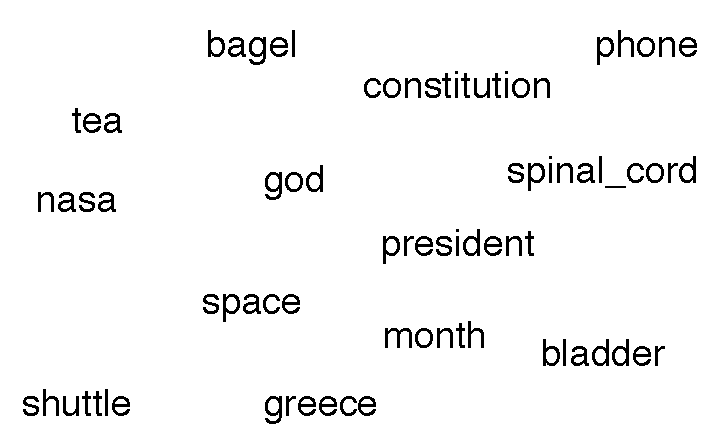
\includegraphics[width=\linewidth]{interactive_topic_models/constraints_1}     }
	\only<3-4>{	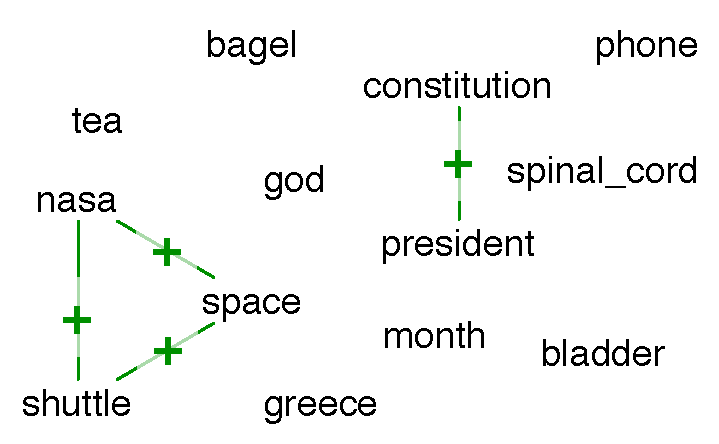
\includegraphics[width=\linewidth]{interactive_topic_models/constraints_2}     }
	\only<5->{	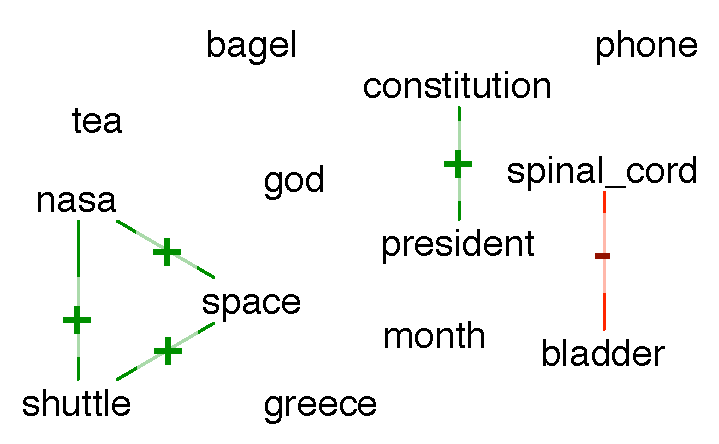
\includegraphics[width=\linewidth]{interactive_topic_models/constraints_3}     }
\end{columns}

}

\ifitmtree

\frame{

	\frametitle{Tree-based Generative Process}

	\begin{itemize}
		\item In LDA, a topic is a multinomial distribution over words
		\item Here, \emph{each topic} is a tree
		\begin{itemize}
			\item Each word is a leaf
			\item Start at root node
			\item Proceed down tree node by node until you reach a leaf
		\end{itemize}
	\end{itemize}
}


\frame{

	\frametitle{Example of Priors}

	\begin{center}
		\only<1>{ 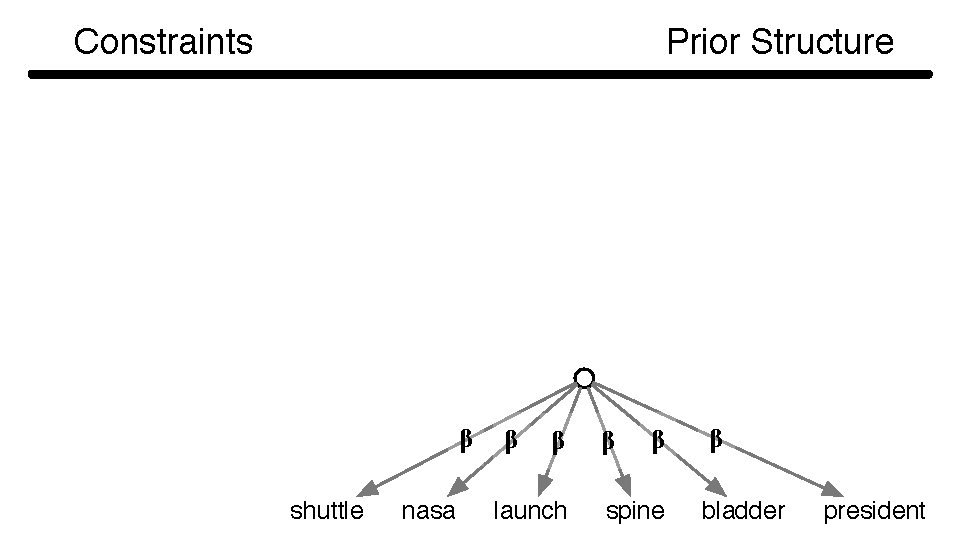
\includegraphics[width=.8\linewidth]{interactive_topic_models/tree_constraints_0} }
		\only<2>{ 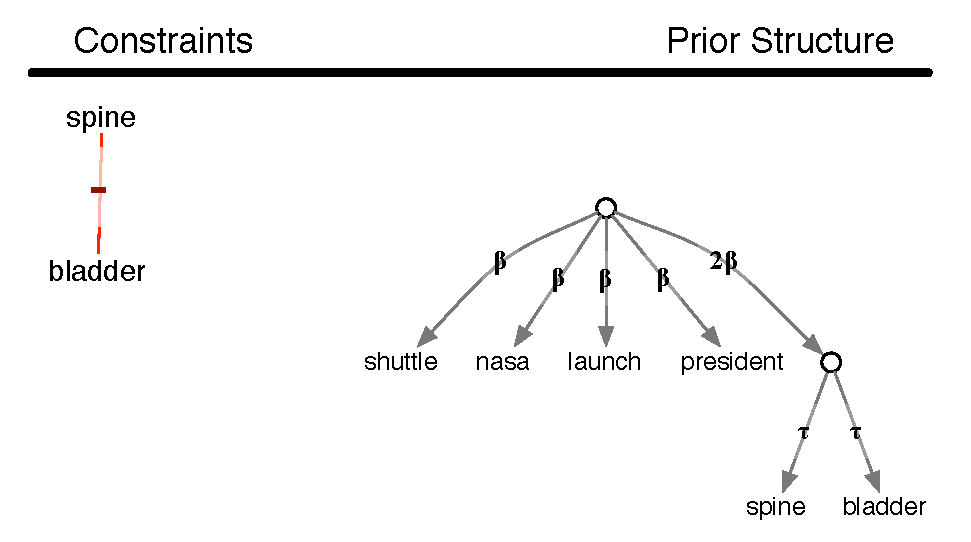
\includegraphics[width=.8\linewidth]{interactive_topic_models/tree_constraints_1} }
		\only<3>{ 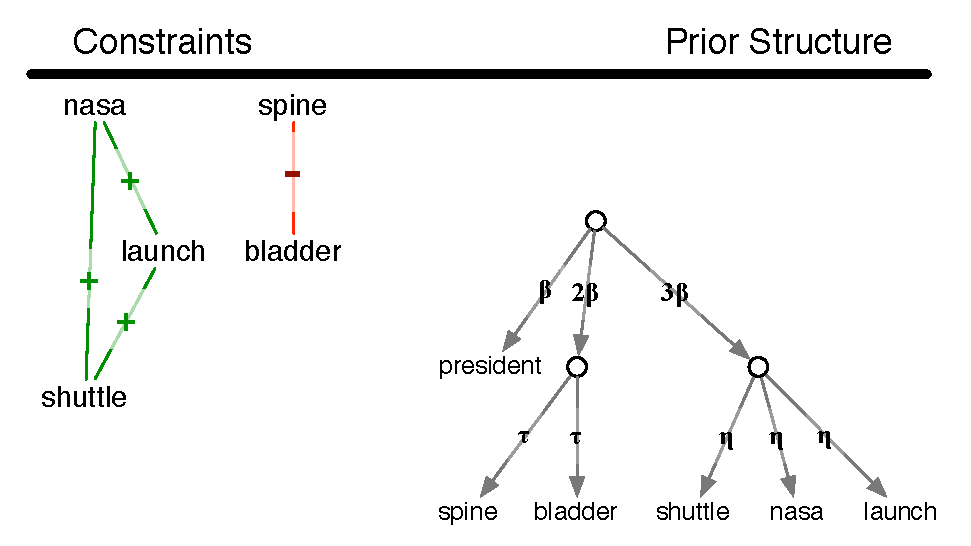
\includegraphics[width=.8\linewidth]{interactive_topic_models/tree_constraints_2} }
	\end{center}

	\begin{columns}

		\column{.5\linewidth}

			\only<2>{

			\begin{itemize}
				\item For negative correlations $\tau << \beta$
				\item Encourages very, very sparse distributions
			\end{itemize}
				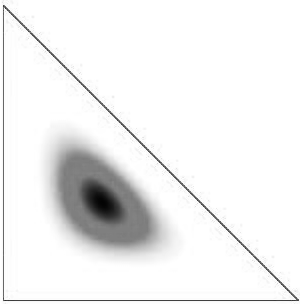
\includegraphics[width=.7\linewidth]{interactive_topic_models/uniform_dirichlet}


			}


			\only<3>{

			\begin{itemize}
				\item For positive correlations $\eta >> \beta$
				\item Encourages uniform distributions
			\end{itemize}
				
\includegraphics[width=.7\linewidth]{interactive_topic_models/sparse_dirichlet}


			}

		\column{.5\linewidth}

	\end{columns}

}

\fi

\frame{
	\frametitle{How to incorporate feedback?}

	\begin{columns}

	\column{.5\linewidth}

		\begin{columns}

			\column{.6\linewidth}

			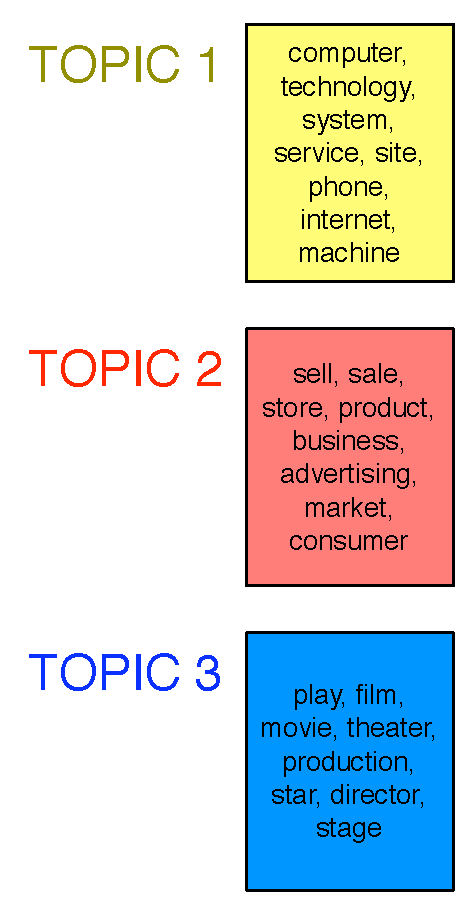
\includegraphics[width=\linewidth]{topic_models/nyt_topics}


			\column{.4\linewidth}
			\begin{center}
				\only<2->{
\includegraphics[width=.6\linewidth]{general_figures/arrow_right_down} \\}
				\only<2->{
\includegraphics[width=.6\linewidth]{general_figures/milkman_dan} \\}
				\invisible<-2>{
\includegraphics[width=.6\linewidth,angle=270]{general_figures/arrow_right_down}}
			\end{center}

		\end{columns}

	\column{.5\linewidth}

	\begin{enumerate}
		\item Fit initial topic modeling
			\pause
		\item Get feedback from user
			\pause
		\item Incrementally relearn model
			\begin{itemize}
				\item Replace the model with a correlated one
				\item Keep computation \alert<4>{fast and consistent}
			\end{itemize}
	\end{enumerate}

	\end{columns}

}



\ifhighlevel

\else

\frame{
	\frametitle{Forgetting is everything}

	\begin{itemize}
		\item Just start over?
			\begin{itemize}
				\item More expensive computation
				\item Might create more problems
				\item Bad user experience
			\end{itemize}
		\item View problem as online inference~\cite{yao-09}
		\item Suggestions reflect errors
		\item ``Forget'' problems
		\item Pretend you're seeing it for the first time
	\end{itemize}
}


\frame{
	\frametitle{Inference}


	\begin{center}

	\only<1> {   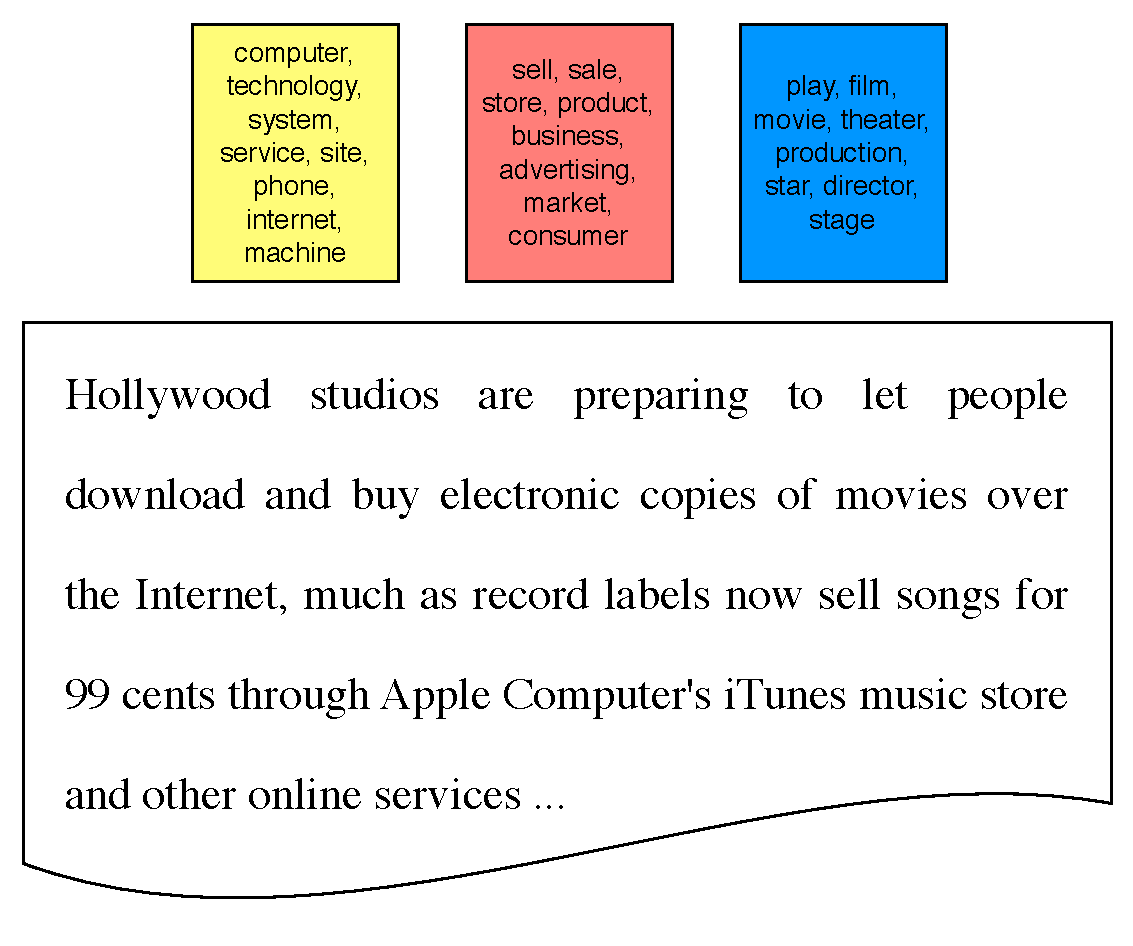
\includegraphics[width=.8\linewidth]{topic_models/inference_0}  }
	\only<2> {   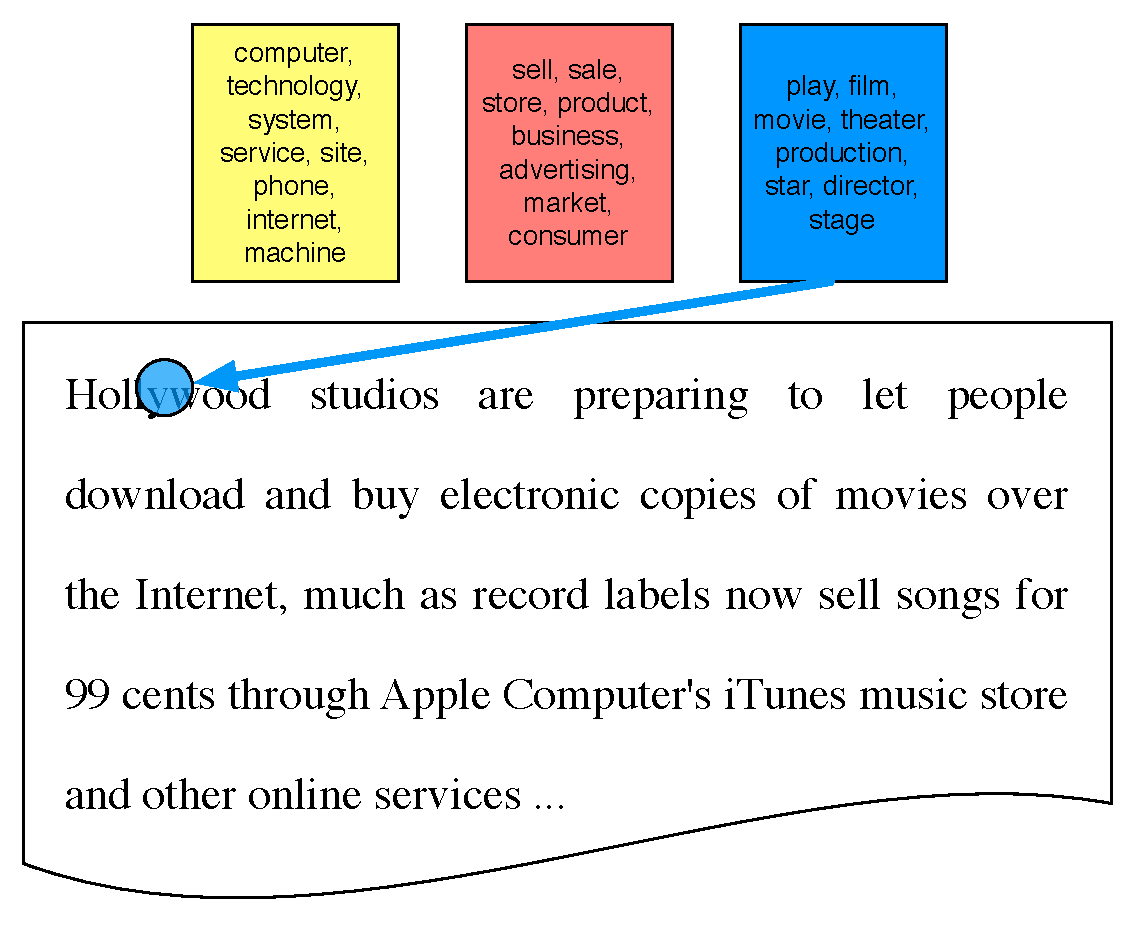
\includegraphics[width=.8\linewidth]{topic_models/inference_1}  }
	\only<3> {   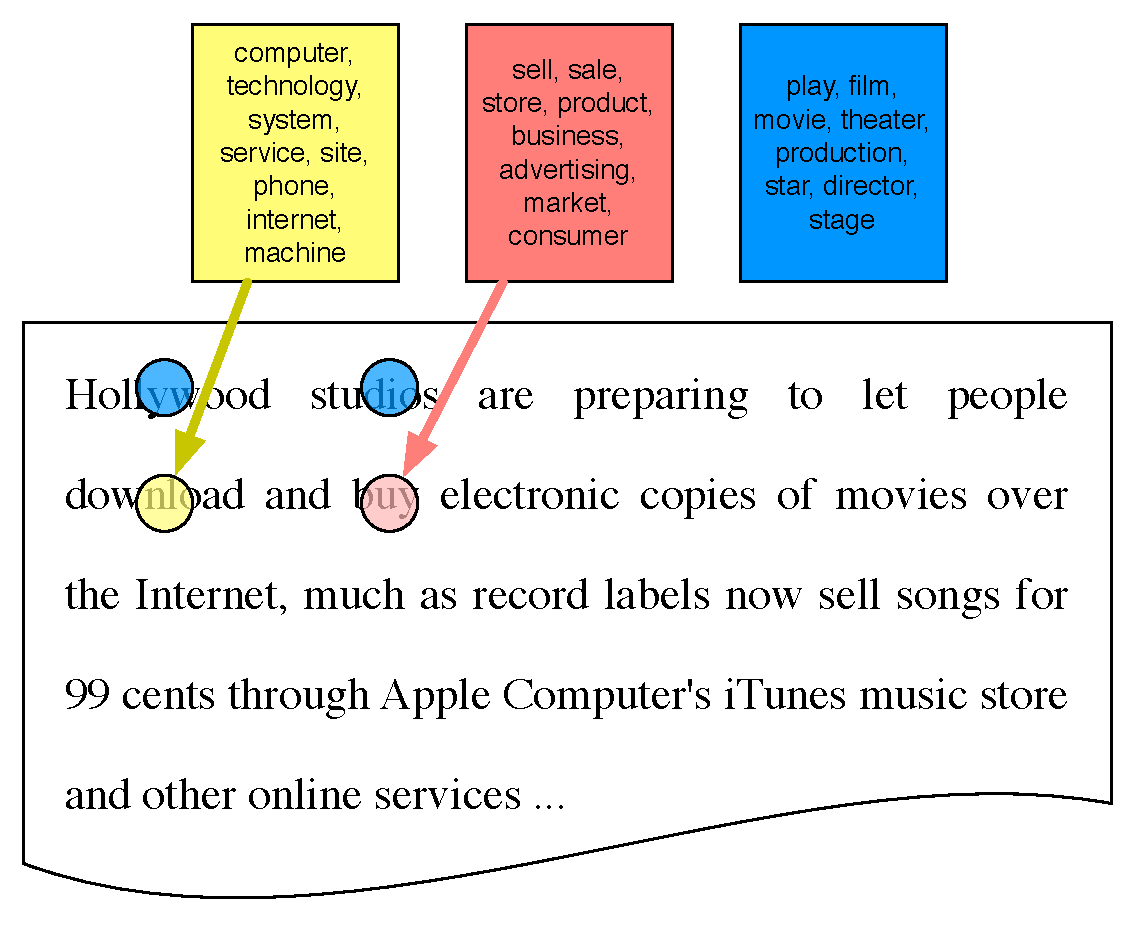
\includegraphics[width=.8\linewidth]{topic_models/inference_2}  }
	\only<4> {   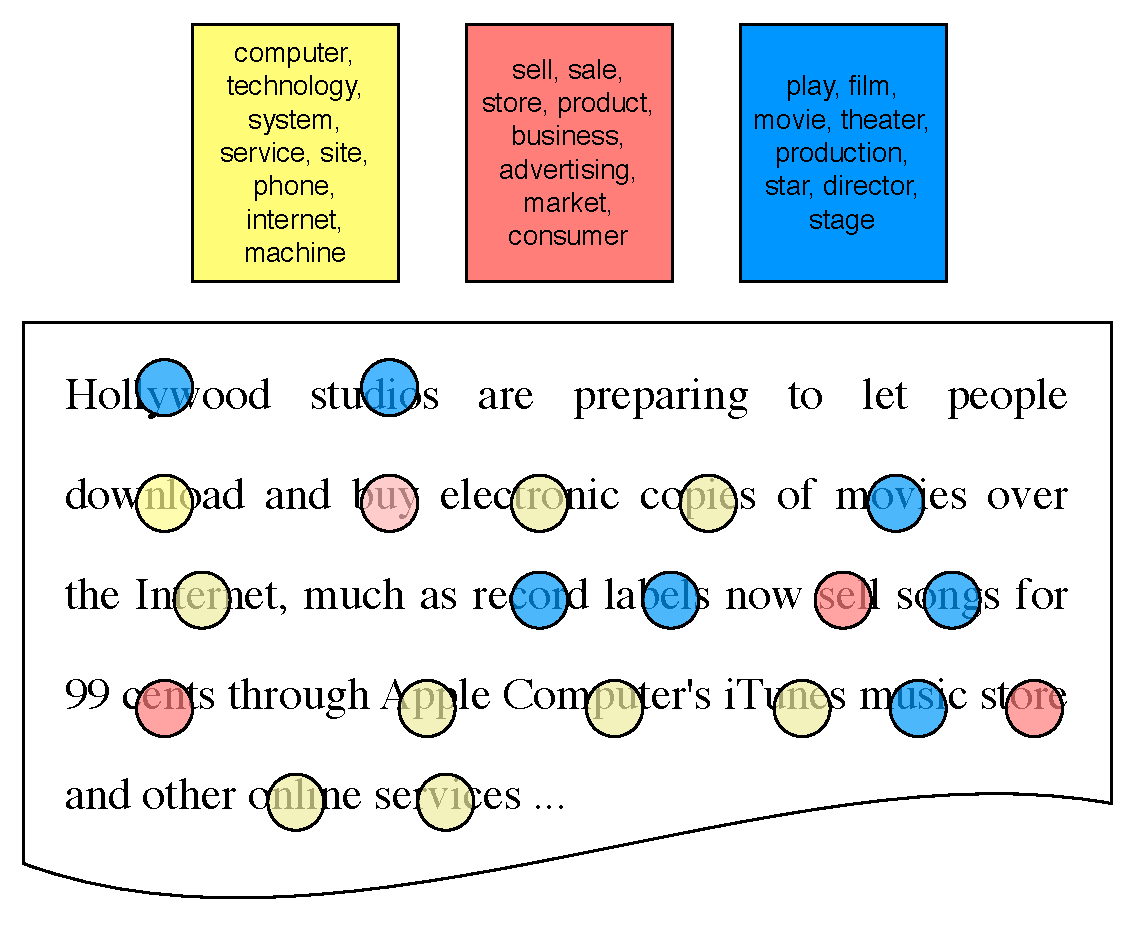
\includegraphics[width=.8\linewidth]{topic_models/inference_3}  }
	\end{center}

}

\frame{
	\frametitle{Inference}

	\begin{columns}

		\column{.5\linewidth}
		\begin{flushright}
			\only<1>{    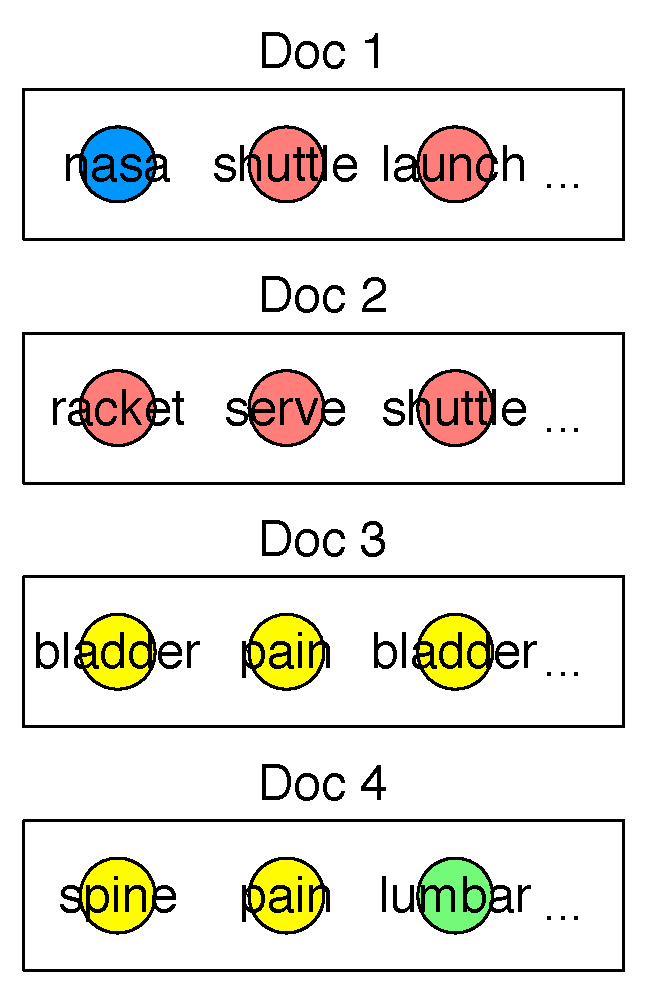
\includegraphics[height=7cm]{interactive_topic_models/mcmc_state_0}    }
			\only<2>{    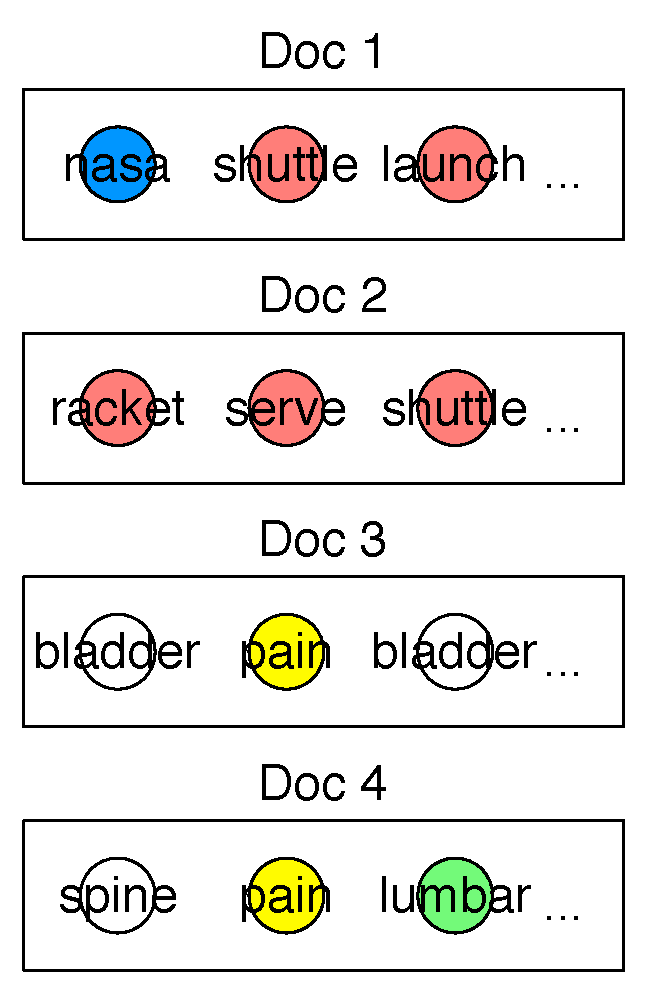
\includegraphics[height=7cm]{interactive_topic_models/mcmc_state_1}    }
			\only<3>{    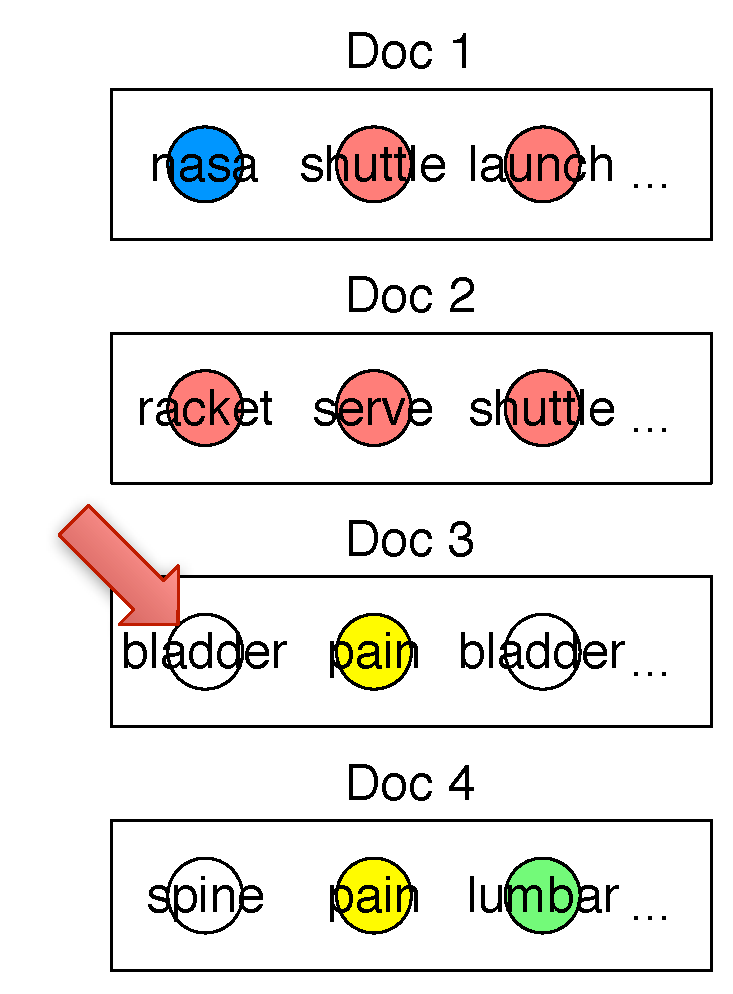
\includegraphics[height=7cm]{interactive_topic_models/mcmc_state_2}    }
			\only<4>{    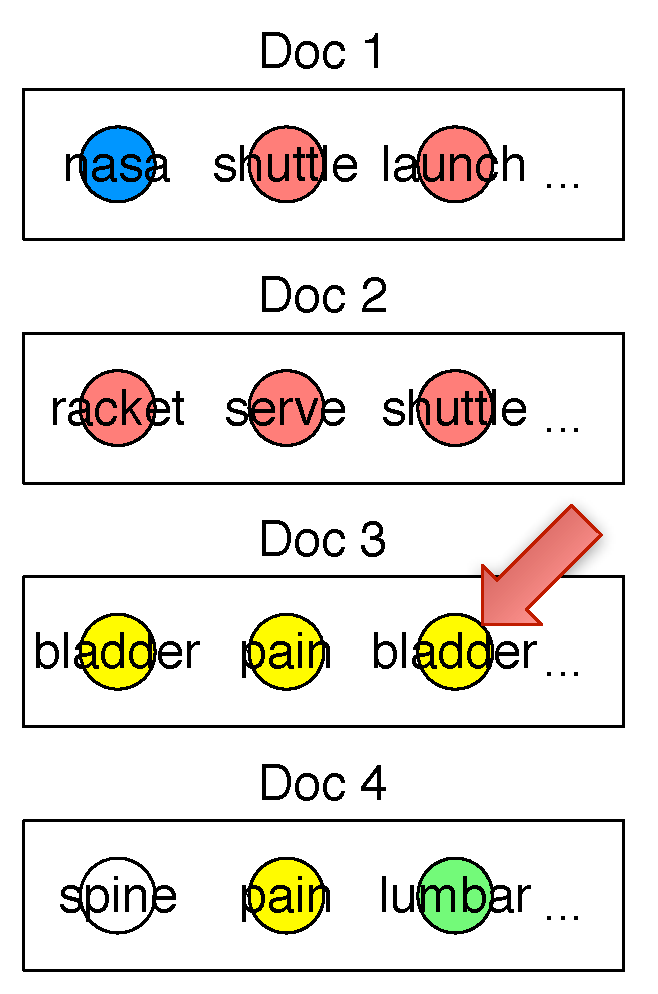
\includegraphics[height=7cm]{interactive_topic_models/mcmc_state_3}    }							\only<5>{    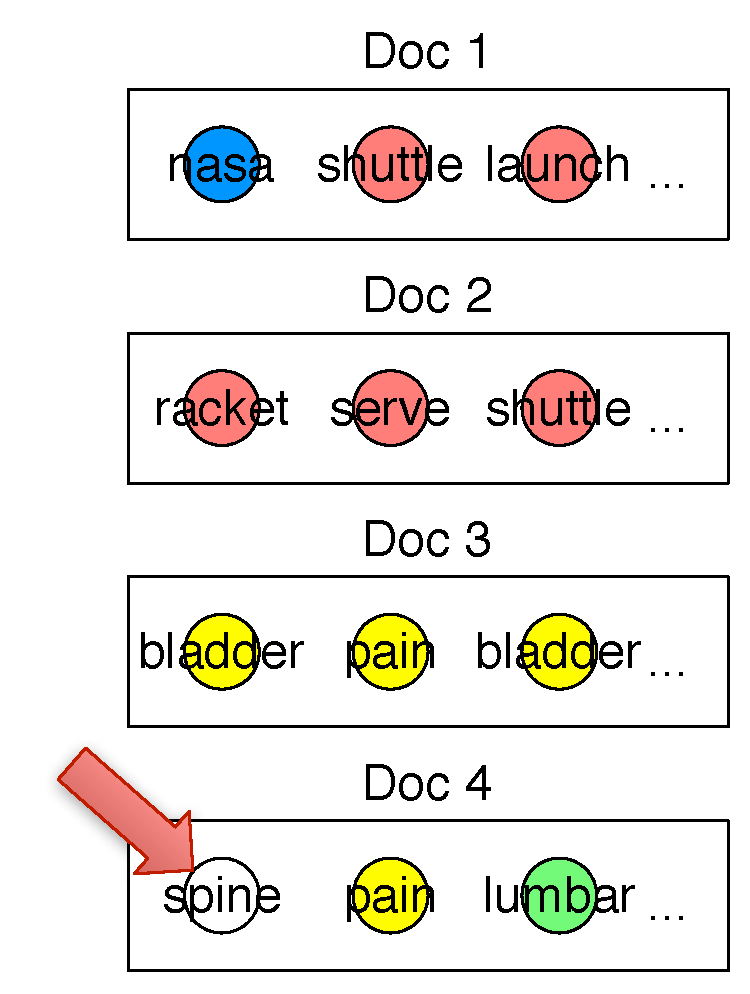
\includegraphics[height=7cm]{interactive_topic_models/mcmc_state_4}    }
			\only<6>{    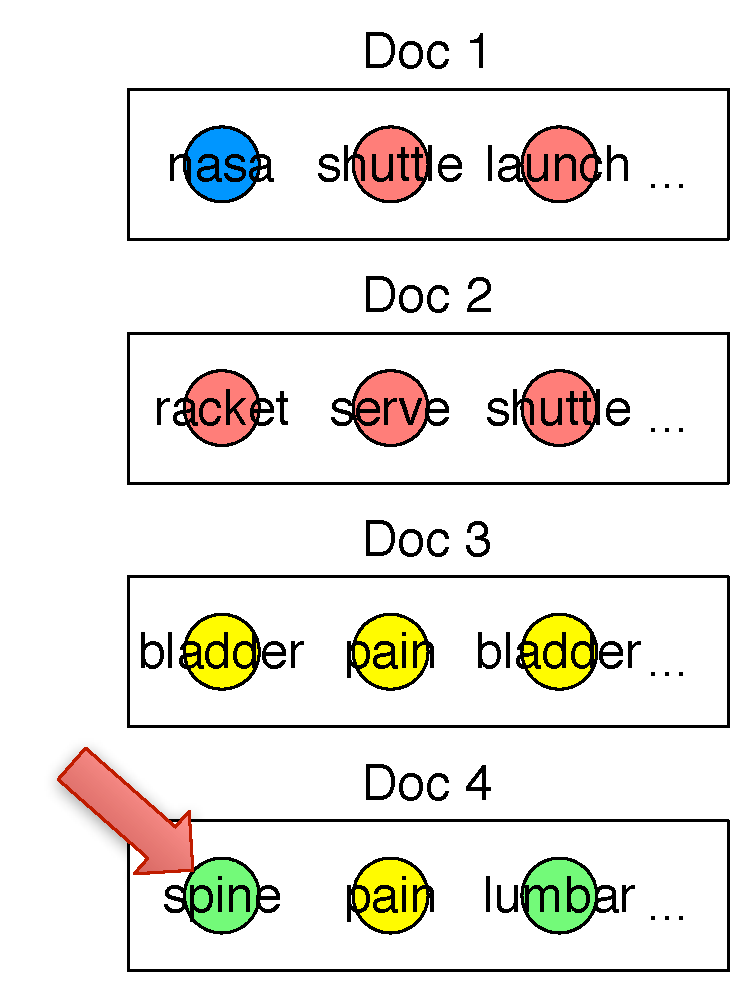
\includegraphics[height=7cm]{interactive_topic_models/mcmc_state_5}    }
			\only<7>{    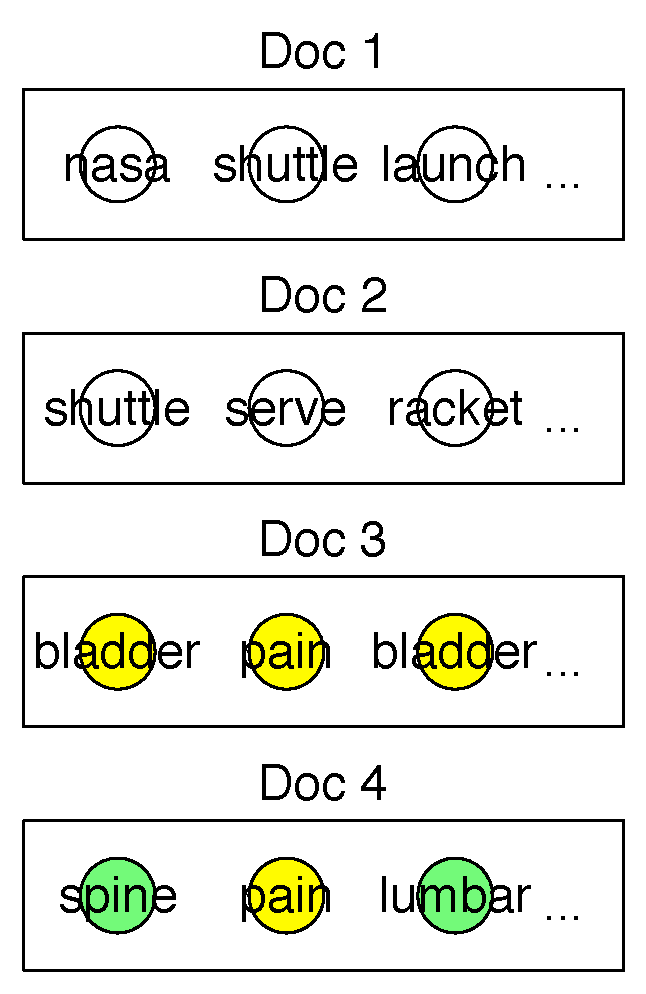
\includegraphics[height=7cm]{interactive_topic_models/mcmc_state_6}    }
			\only<8>{    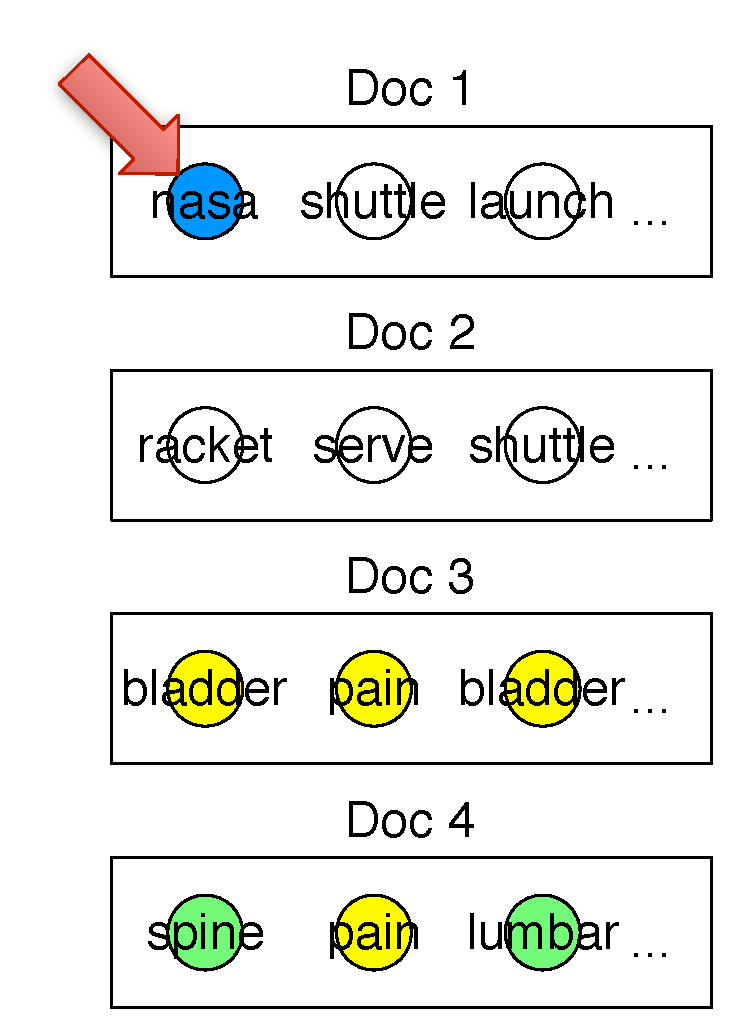
\includegraphics[height=7cm]{interactive_topic_models/mcmc_state_7}    }
			\only<9>{    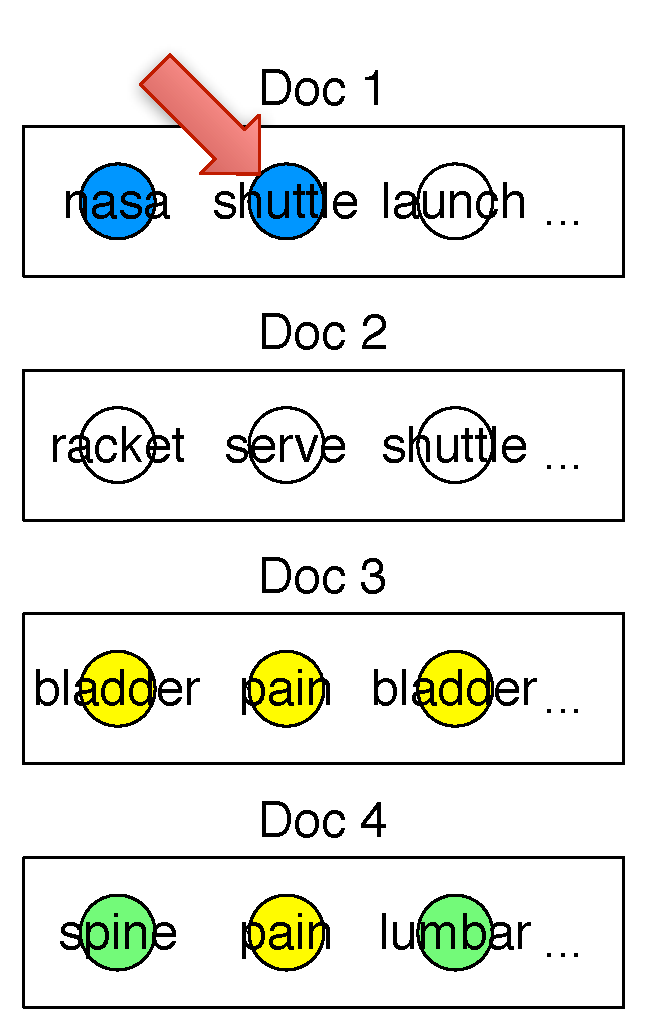
\includegraphics[height=7cm]{interactive_topic_models/mcmc_state_8}    }
			\only<10>{    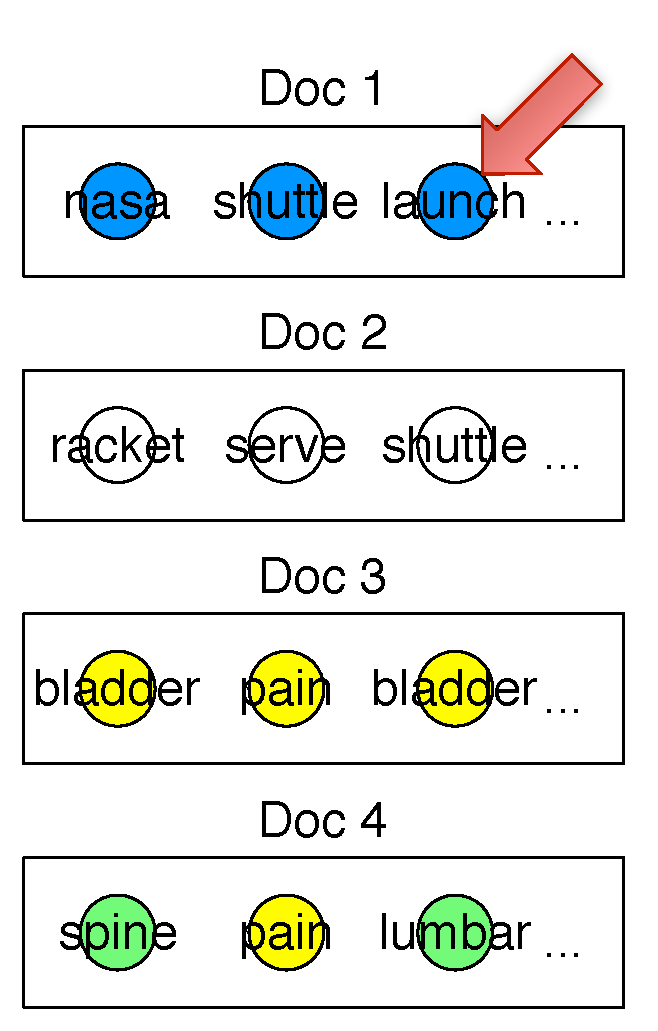
\includegraphics[height=7cm]{interactive_topic_models/mcmc_state_9}    }							\only<11->{    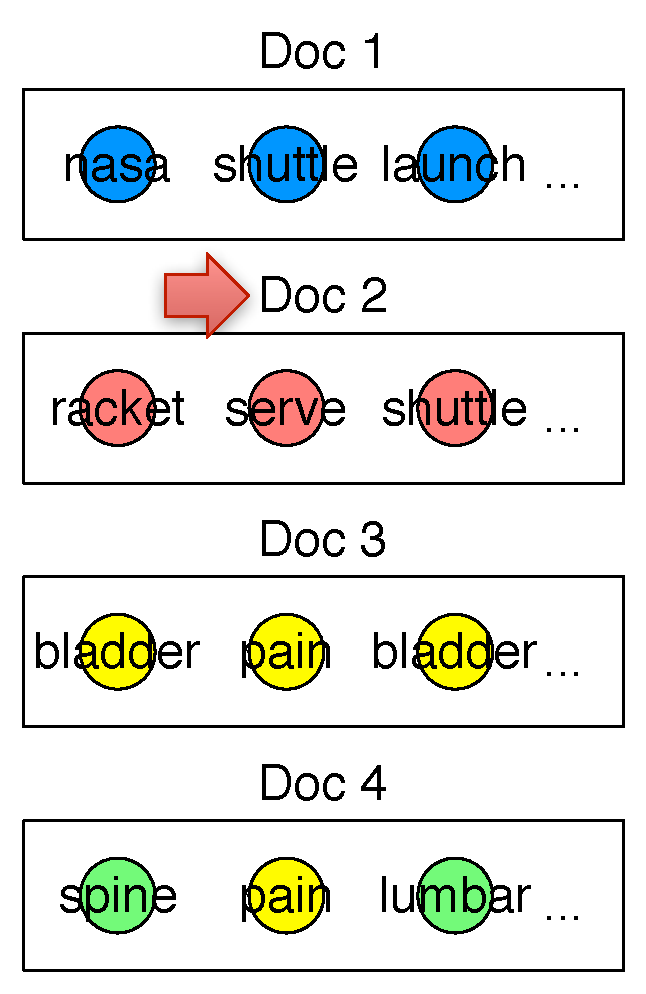
\includegraphics[height=7cm]{interactive_topic_models/mcmc_state_a}    }
		\end{flushright}
		\column{.5\linewidth}

		\only<1> {  This toy example has all the problems from before!  }
		\only<2-6> {

		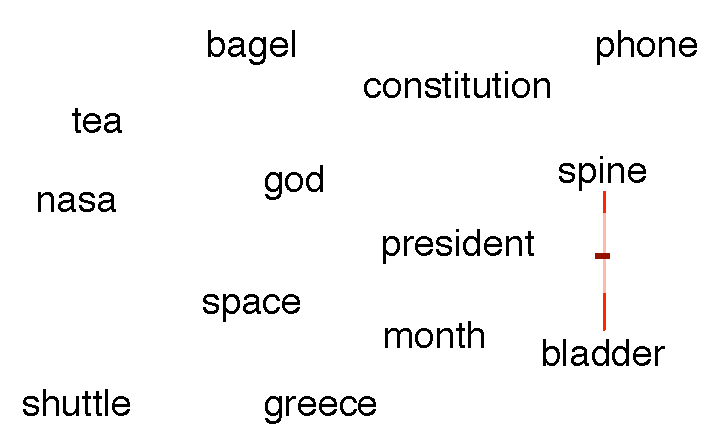
\includegraphics[width=\linewidth]{interactive_topic_models/constraints_4}

		\begin{block}{Negative Correlation}

		\begin{itemize}
			\item \emph{bladder} and \emph{spine} can't be together
			\item Idea 1: Forget {\bf terms}
		\end{itemize}


		\end{block}

		}

		\only<7-11> {

		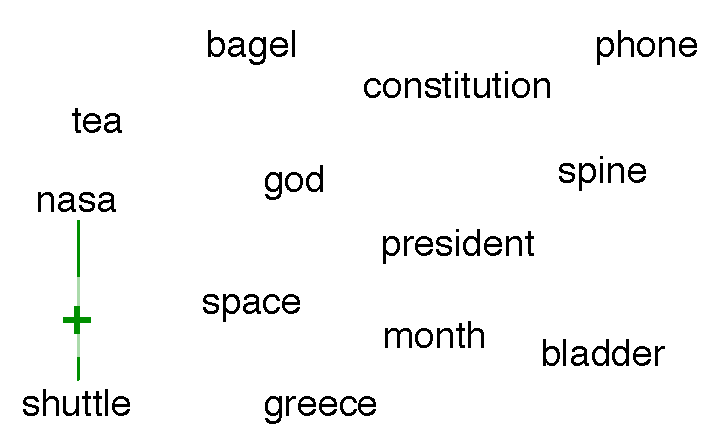
\includegraphics[width=\linewidth]{interactive_topic_models/constraints_5}

		\begin{block}{Positive Correlation}
		\begin{itemize}
			\item \emph{shuttle} and \emph{nasa} should be together
			\item Idea 2: Forget {\bf documents} with terms
		\end{itemize}
		\end{block}

		}

	\end{columns}

}


\frame{
	\frametitle{Tricky details}

	\begin{itemize}
		\item Overlapping correlations
		\begin{itemize}
			\item Are positive correlations transitive (polysemy)
			\item Overlapping negative correlations require computing maximal cliques in complement graph
		\end{itemize}
		\item How do you do hyperparameter optimization?
		\pause
		\item For the rest of this talk, only {\bf positive} correlations and preset hyper parameters
	\end{itemize}
}

\fi

\renewcommand{\tb}[1]{\parbox{0.8\linewidth}{ \tiny{ #1 }} \vspace{.2cm} }

\frame{

\vspace{-1cm}

\begin{columns}

\column{.5\linewidth}

\begin{tabular}{l*{2}{c}r}
	Topic & Before \\
\hline

\alert<2>{{\bf 1}} & \tb{ \alert<2>{election, yeltsin, russian, political, party, democratic, russia,
  president, democracy, boris, country, south, years, month, government, vote,
  since, leader, presidential, military} } \\

2 & \tb{new, york, city, state, mayor, budget, giuliani, council, cuomo, gov,
  plan, year, rudolph, dinkins, lead, need, governor, legislature, pataki,
  david} \\

3 & \tb{nuclear, arms, weapon, defense, treaty, missile, world, unite, yet,
  soviet, lead, secretary, would, control, korea, intelligence, test, nation,
  country, testing} \\

4 & \tb{president, bush, administration, clinton, american, force, reagan, war,
  unite, lead, economic, iraq, congress, america, iraqi, policy, aid,
  international, military, see} \\

& \vdots \\

\alert<2>{{\bf 20}} & \tb{\alert<2>{soviet, lead, gorbachev, union, west, mikhail, reform, change, europe,
  leaders, poland, communist, know, old, right, human, washington, western,
  bring, party} }\\

\end{tabular}

\column{.5\linewidth}

\only<3> {

	\begin{block}{Suggestion}
	\emph{boris, communist, gorbachev, mikhail, russia,
  russian, soviet, union, yeltsin }
	\end{block}

}

\only<4-> {

\begin{tabular}{l*{2}{c}r}
	Topic & After \\
\hline

\alert<5>{{\bf 1}} & \alert<5>{\tb{election, democratic, south, country, president, party, africa, lead,
  even, democracy, leader, presidential, week, politics, minister, percent,
  voter, last, month, years} } \\

\alert<6>{2} & \tb{new, york, city, state, mayor, budget, council, giuliani, gov, cuomo,
  year, rudolph, dinkins, legislature, plan, david, governor, pataki, need, cut}
\\

\alert<6>{3} & \tb{nuclear, arms, weapon, treaty, defense, war, missile, may, come, test,
  american, world, would, need, lead, get, join, yet, clinton, nation} \\

\alert<6>{4} & \tb{president, administration, bush, clinton, war, unite, force, reagan,
  american, america, make, nation, military, iraq, iraqi, troops, international,
  country, yesterday, plan} \\

   & \vdots \\

\alert<4>{ {\bf 20} } & \alert<4> {\tb{soviet, union, economic, reform, yeltsin, russian, lead, russia,
  gorbachev, leaders, west, president, boris, moscow, europe, poland, mikhail,
  communist, power, relations} } \\

\end{tabular}

}

\end{columns}

}

\providecommand{\blue}[1]{{\color{blue}{#1}}}
\providecommand{\red}[1]{{\color{red}{#1}}}
\providecommand{\green}[1]{{\color{green}{#1}}}

\begin{frame}

\frametitle{Example: Negative Constraint}

\begin{columns}

\column{.4\linewidth}

\begin{tabular}{l*{2}{c}r}
	Topic & Words \\
\hline

{\bf 318} & \tb{\red{bladder}, sci, \blue{spinal\_cord}, \blue{spinal\_cord\_injury}, \blue{spinal}, \red{urinary}, \red{urinary\_tract}, \red{urothelial},\blue{injury}, \blue{motor}, \blue{recovery}, \blue{reflex}, \blue{cervical}, \red{urothelium}, \blue{functional\_recovery}} \\

\end{tabular}

\column{.1\linewidth}

\column{.4\linewidth}

\only<3->{
\begin{tabular}{l*{2}{c}r}
	Topic & Words \\
\hline

{\bf 318} & \tb{sci, \blue{spinal\_cord}, \blue{spinal\_cord\_injury}, \blue{spinal}, \blue{injury}, \blue{recovery}, \blue{motor}, \blue{reflex}, \red{urothelial}, \green{injured}, \blue{functional\_recovery}, \green{plasticity}, \green{locomotor}, \blue{cervical}, \green{locomotion}}\\

\end{tabular}
}

\end{columns}

\only<2->{
\begin{block}{Negative Constraint}
  spinal\_cord, bladder
\end{block}

}

\end{frame}




\begin{frame}

        \frametitle{Experiments}

\begin{columns}

\column{.5\linewidth}

  \begin{itemize}
   \item Simulating users through classifying social media
     \begin{itemize}
       \item Investigating different learning strategies
       \item How much to forget
     \end{itemize}
   \end{itemize}

\column{.5\linewidth}

\begin{center}
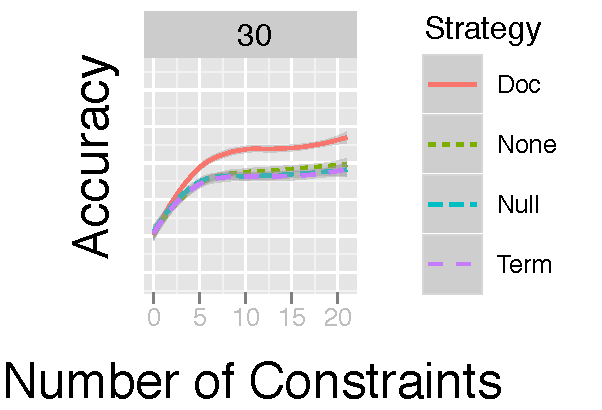
\includegraphics[width=\linewidth]{interactive_topic_models/ablation_30_topics}
\end{center}

\end{columns}

\begin{itemize}
    \item User study: mechanical Turk
      \begin{itemize}
        \item We can't do everything users want: proper names, mac vs. pc
        \item Users are senstive to polysemy (``msg'': food or e-mail)
      \end{itemize}
    \item User study: exploring congressional debates
      \begin{itemize}
        \item Collaboration with social scientists
        \item Interactivity makes people use topic models more
       \end{itemize}
  \end{itemize}


\end{frame}

% -------------------------
% Old version

% \frame{
% 	\frametitle{Interactive Topic Models in the Wild \dots}
% \begin{center}
% 	\only<1>{    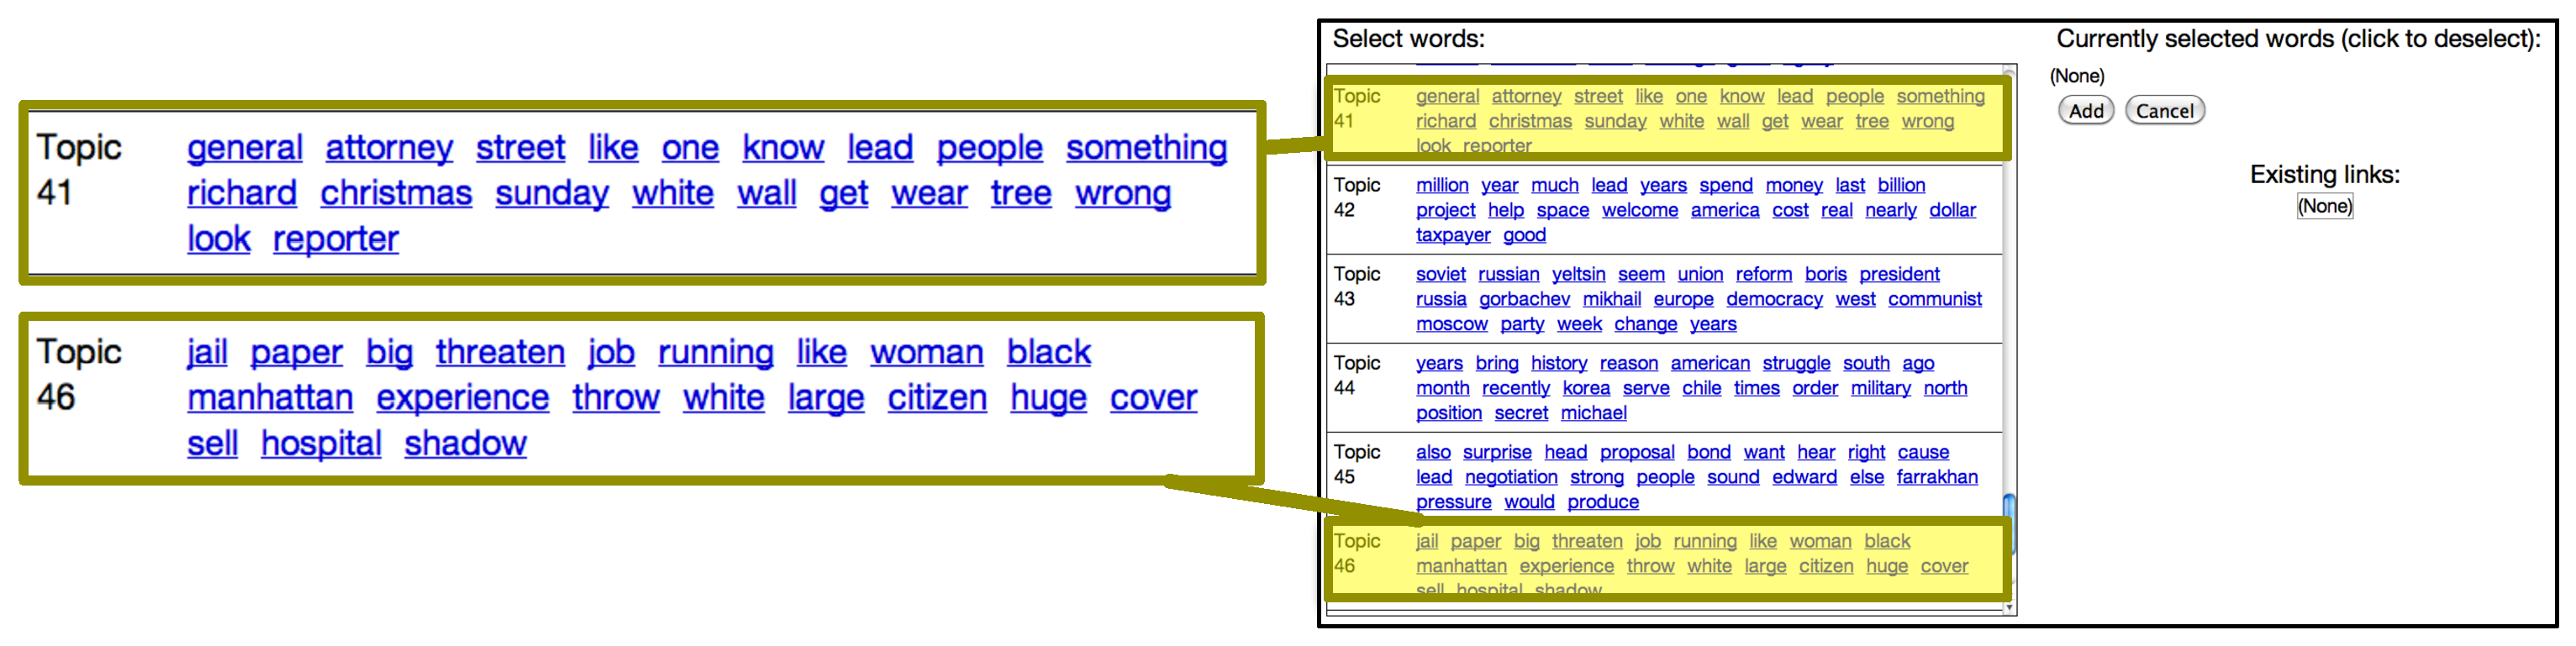
\includegraphics[width=\linewidth]{interactive_topic_models/turk_topic}    }
% 	\only<2>{    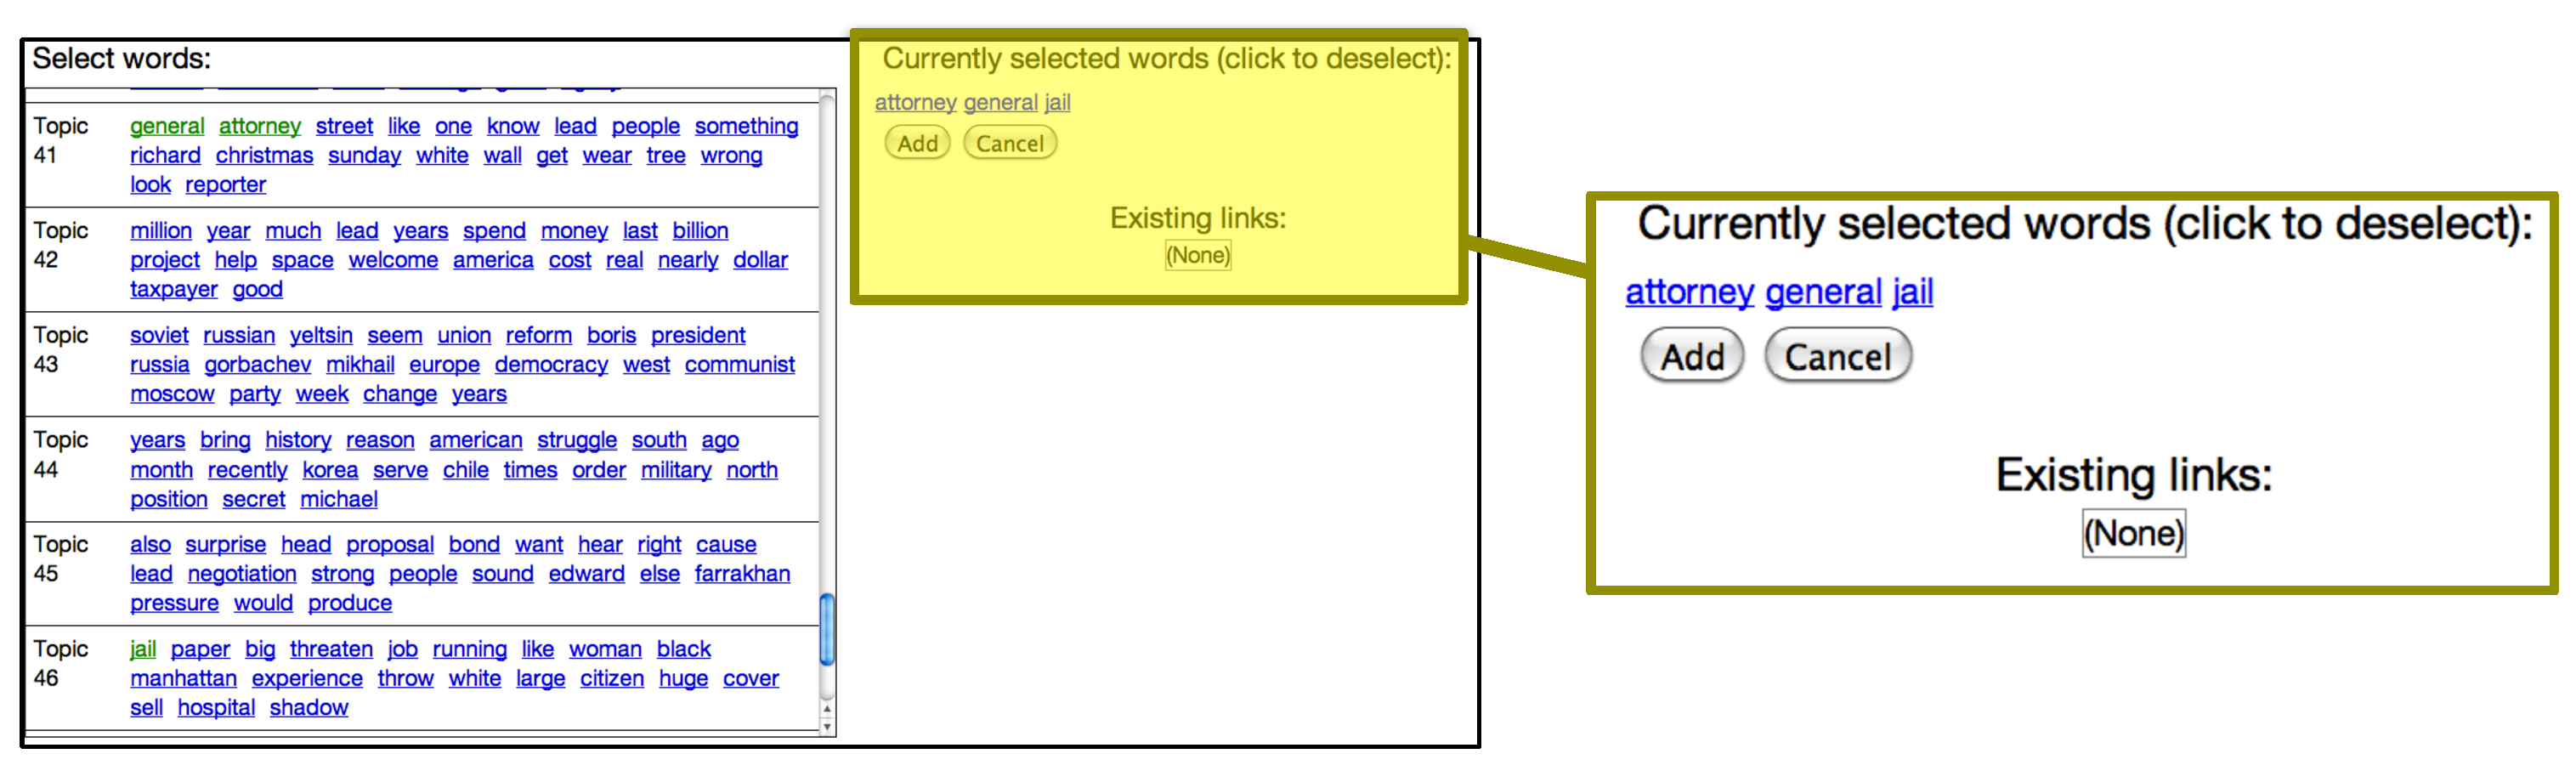
\includegraphics[width=\linewidth]{interactive_topic_models/turk_sel_constraint}    }
% 	\only<3>{    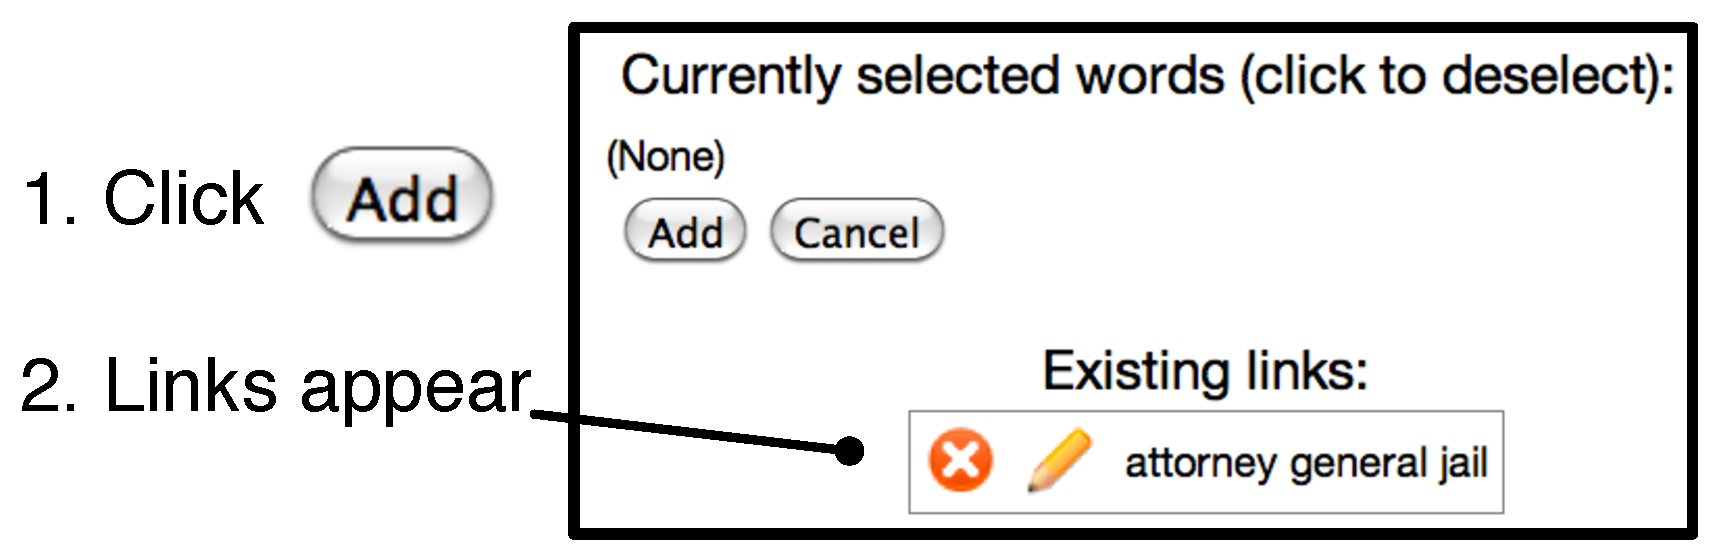
\includegraphics[width=\linewidth]{interactive_topic_models/turk_add_link}    }
% 	\only<4>{    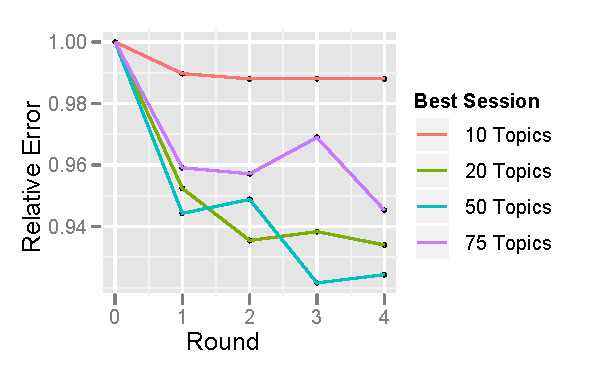
\includegraphics[width=\linewidth]{interactive_topic_models/best_mturk_rel_error}    }

% 	\begin{block}{}
% 		Documents were 20 Newsgroups
% 	\end{block}
% \end{center}
% }



\iflong

\frame{
	\frametitle{What people did \dots}


	\begin{itemize}
		\item Inscrutable
			\begin{itemize}
				\item better, people, right, take, things
				\item fbi, let, says
			\end{itemize}
		\item Collocations
			\begin{itemize}
				\item jesus, christ
				\item solar, sun
				\item even, number
				\item book, list
			\end{itemize}
		\item Common instances (e.g. first names)
		\item Not all were successful: mac, windows

	\end{itemize}

}


\frame{

	\frametitle{Future steps}

	\begin{itemize}
		\item Speeding up
		\item Suggesting correlations
		\item Incorporating other domain knowledge
		\item Interactive vocabulary
		\item Other domains
		\item Incorporating this analysis in other models
	\end{itemize}

}

\fi


